\subsection{Quagga Install}\label{quagga-install-and-configuration}

\subsubsection{Download Quagga:}\label{download-quagga}

\begin{quote}
http://download.savannah.gnu.org/releases/quagga/quagga-1.2.1.tar.gz
\end{quote}

\subsubsection{Unzip and Configure:}\label{unzip-and-configure}

\begin{quote}
\$ ./configure --enable-vtysh --enable-user=root --enable-group=root --enable-vty-group=root
\end{quote}

If GNU awk is required:

\begin{quote}
\$ sudo apt-get install gawk
\end{quote}

If libreadline is required:

\begin{quote}
\$ sudo apt-get install libreadline6 libreadline6-dev
\end{quote}

If libcares is required:

\begin{quote}
\$ sudo apt-get install libc-ares-dev
\end{quote}

\subsubsection{Make:}\label{make}

\begin{quote}
\$ make
\end{quote}

If aclocal-1.15 is missing:

\begin{quote}
\$ sudo apt-get install automake
\end{quote}

If makeinfo is missing:

\begin{quote}
\$ sudo apt-get install texinfo
\end{quote}

\subsubsection{Make install:}\label{make-install}

\begin{quote}
\$ sudo make install
\end{quote}

\subsubsection{Make new file, copy zebra.conf.sample to
zebra.conf:}\label{make-new-file-copy-zebra.conf.sample-to-zebra.conf}

\begin{quote}
\$ cd /usr/local/etc
\end{quote}

\begin{quote}
\$ sudo cp zebra.conf.sample zebra.conf
\end{quote}

\subsubsection{Quagga(Zebra) Service
Start:}\label{quaggazebra-service-start}

\begin{quote}
\$ sudo zebra -d
\end{quote}

If zebra: error while loading shared libraries: libzebra.so.1: cannot open shared object file: No such file or directory

\begin{quote}
\$ cd /usr/local/lib
\end{quote}

\begin{quote}
\$ sudo cp libzebra.* /lib
\end{quote}

\begin{quote}
\$ sudo rm libzebra.*
\end{quote}

\subsubsection{Connect to zebra using telnet(password
zebra):}\label{connect-to-zebra-using-telnetpassword-zebra}

\begin{quote}
\$ telnet localhost 2601
\end{quote}

\subsection{Ping Test on OSPF Experiment (One Mininet)}\label{run-ospf-experiment-one-mininet}

\subsubsection{Experiment Topo:}\label{experiment-topo}

\begin{figure}[h]
\centering
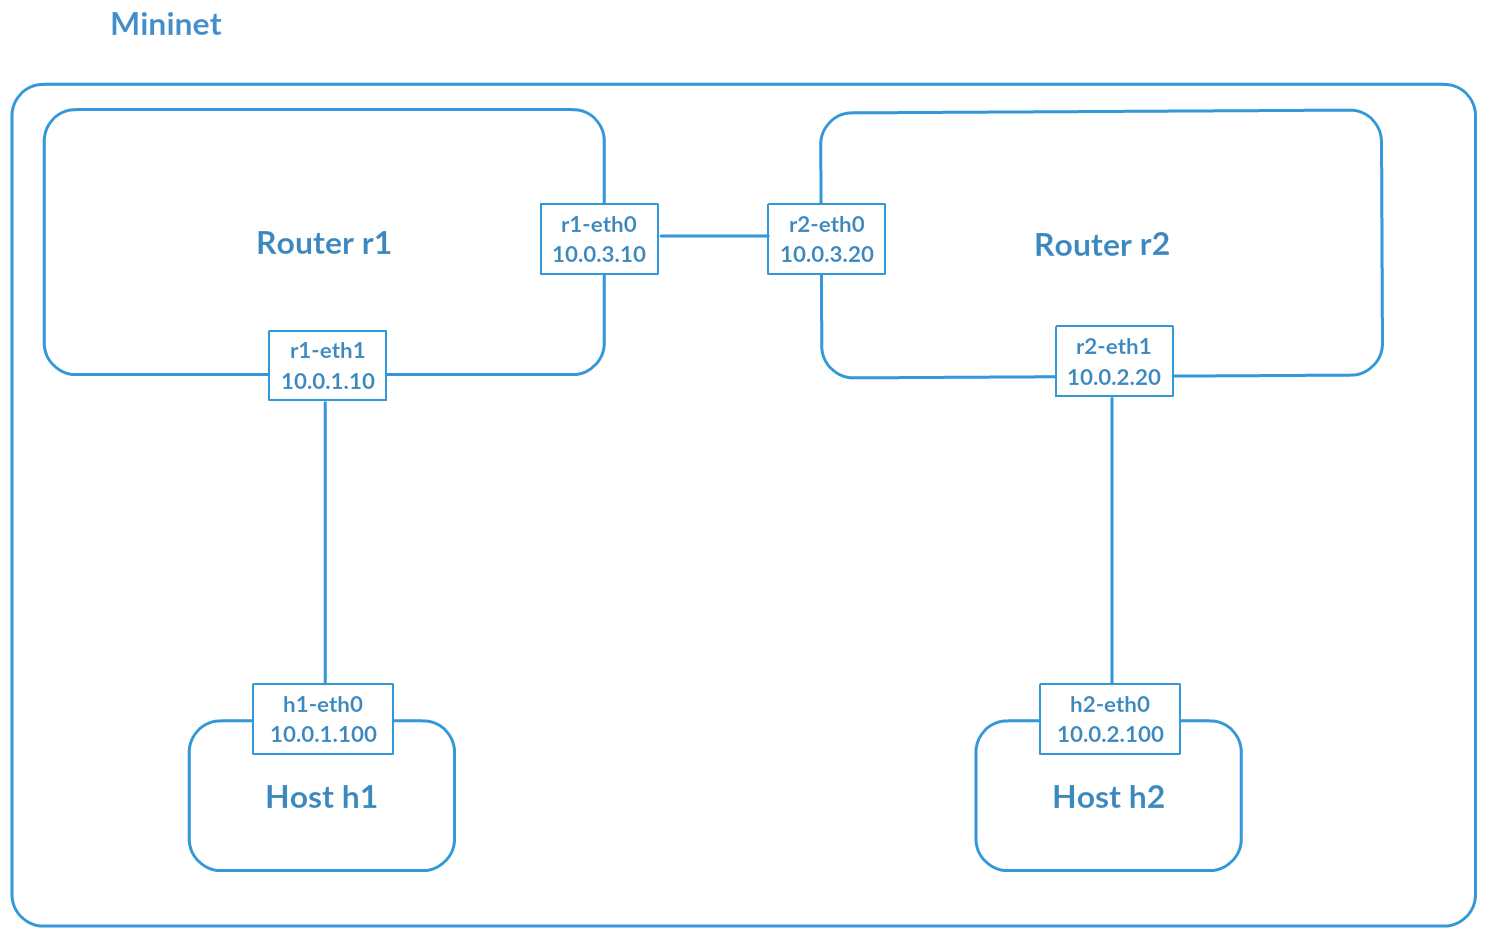
\includegraphics[width=0.8\textwidth]{./Figure/Topo/Exp1.png}
\caption{Ping Test on OSPF Experiment (One Mininet) \label{fig:Exp1}}
\end{figure}

\subsubsection{Create Zebra Configuration File for router r1 and r2:}\label{create-zebra-configuration-file-for-router-r1-and-r2}

\begin{quote}
\$ cd /usr/local/etc
\end{quote}

\begin{quote}
\$ cp zebra.conf.sample r1zebra.conf
\end{quote}

\begin{quote}
\$ cp zebra.conf.sample r2zebra.conf
\end{quote}

\subsubsection{Create OSPF Configuration File for router r1 and
r2:}\label{create-ospf-configuration-file-for-router-r1-and-r2}

\begin{quote}
\$ cd /usr/local/etc
\end{quote}

\begin{quote}
\$ cp ospfd.conf r1ospfd.conf
\end{quote}

\begin{quote}
\$ cp ospfd.conf r2ospfd.conf
\end{quote}

\subsubsection{Edit OSPF configuration
File:}\label{edit-ospf-configuration-file}

Edit r1ospfd.conf

\begin{verbatim}
hostname r1_ospfd
password 123
enable password 123

router ospf
  ospf router-id 10.0.3.10
  network 10.0.3.0/24 area 0
  network 10.0.1.0/24 area 0
debug ospf event
log file /usr/local/etc/r1ospfd.log
\end{verbatim}

Edit r2ospfd.conf

\begin{verbatim}
hostname r2_ospfd
password 123
enable password 123

router ospf
  ospf router-id 10.0.3.20
  network 10.0.3.0/24 area 0
  network 10.0.2.0/24 area 0
debug ospf event
log file /usr/local/etc/r2ospfd.log
\end{verbatim}

\subsubsection{Start Mininet Script:}\label{start-mininet-script}

\begin{quote}
\$ sudo python QuaggaOSPF.py
\end{quote}

\subsubsection{Ping test:}\label{ping-test}

\begin{quote}
mininet\textgreater{} pingall
\end{quote}

It may take a while(40s) to add route.

\subsection{Ping Test on OSPF Experiment (Hybrid)}\label{run-ospf-experiment-hybrid}

\subsubsection{Experiment Topo:}\label{experiment-topo-1}

\begin{figure}[h]
\centering
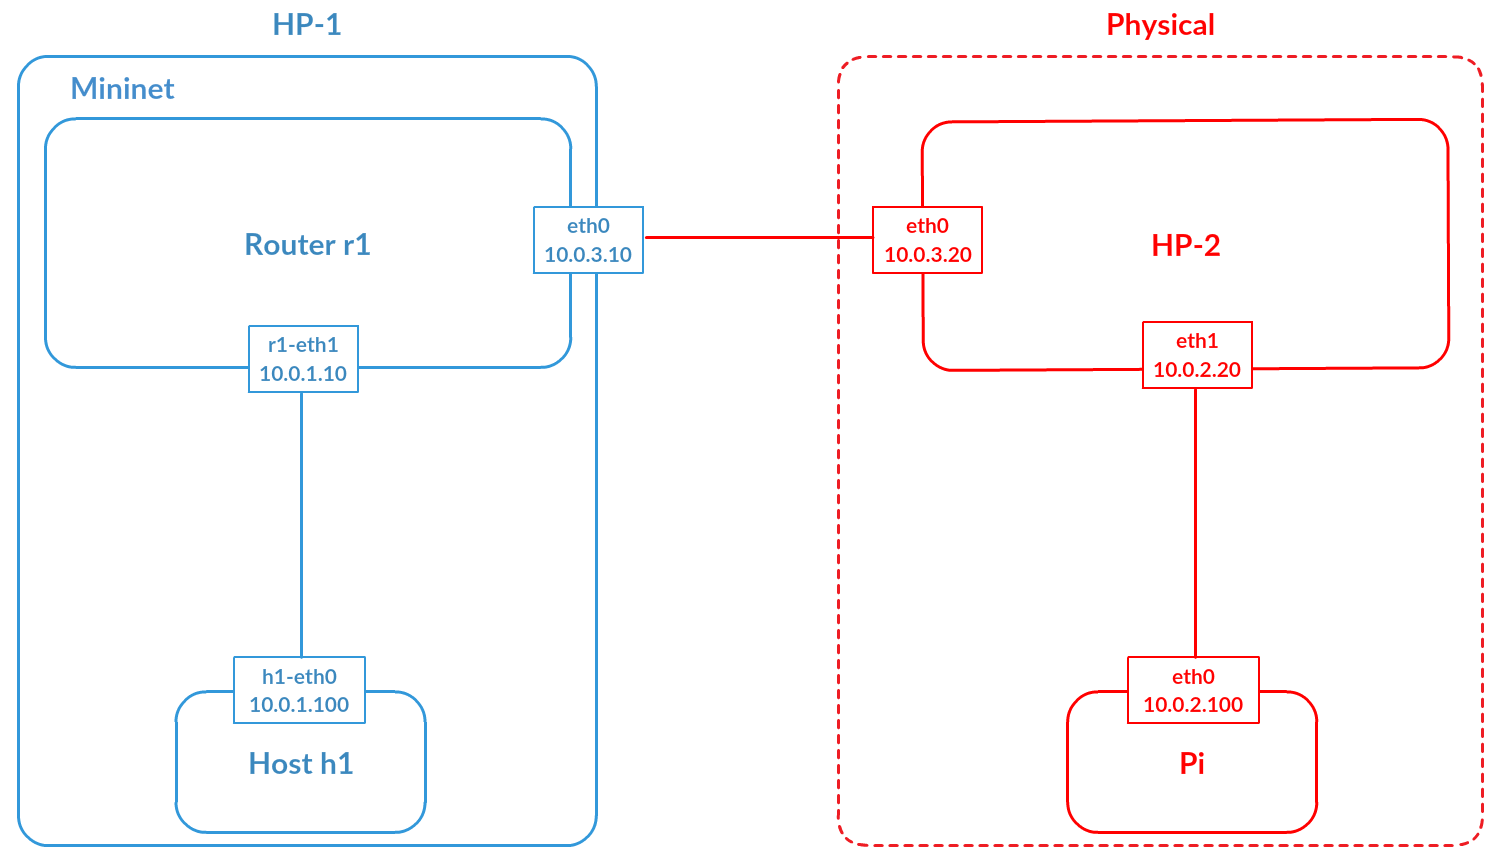
\includegraphics[width=0.8\textwidth]{./Figure/Topo/Exp2.png}
\caption{Ping Test on OSPF Experiment (Hybrid) \label{fig:Exp2}}
\end{figure}

\subsubsection{Run Mininet Script on PC1:}\label{run-mininet-script-on-pc1}

\begin{quote}
\$ sudo python QuaggaOSPF (hybrid).py
\end{quote}

\subsubsection{Copy Zebra Configuration File on
PC2:}\label{copy-zebra-configuration-file-on-pc2}

\begin{quote}
\$ cp zebra.conf.sample zebra.conf
\end{quote}

\subsubsection{Copy and Edit OSPF Configuration File on
PC2:}\label{copy-and-edit-ospf-configuration-file-on-pc2}

\begin{quote}
\$ cd /usr/local/etc
\end{quote}

\begin{quote}
\$ cp ospfd.conf.sample ospfd.conf
\end{quote}

\begin{quote}
\$ nano ospfd.conf
\end{quote}

\begin{adjustwidth}{1cm}{0cm}
\begin{verbatim}
hostname hp2_ospfd
password 123
enable password 123

router ospf
 ospf router-id 10.0.3.20
 network 10.0.3.0/24 area 0
 network 10.0.2.0/24 area 0
\end{verbatim}
 \end{adjustwidth}

\subsubsection{Run Zebra and OSPF on PC2:}\label{run-zebra-and-ospf-on-pc2}

\begin{quote}
\$ sudo zebra -d
\end{quote}

\begin{quote}
\$ sudo ospfd -d
\end{quote}

\subsubsection{Configure IP address and gateway on
Pi:}\label{configure-ip-address-and-gateway-on-pi}

\begin{quote}
\$ sudo ifconfig eth0 10.0.2.100/24
\end{quote}

\begin{quote}
\$ sudo route add default gw 10.0.2.20
\end{quote}

\subsubsection{Ping Test:}\label{ping-test-1}

\begin{quote}
mininet\textgreater{} h1 ping 10.0.2.100
\end{quote}

It may take a while(40s) to add route.

\subsection{Ping Test on SDN and Non-SDN Combination Experiment}\label{run-sdn-and-non-sdn-combination-experiment}

\subsubsection{Experiment Topo:}\label{experiment-topo-2}

\begin{figure}[h]
\centering
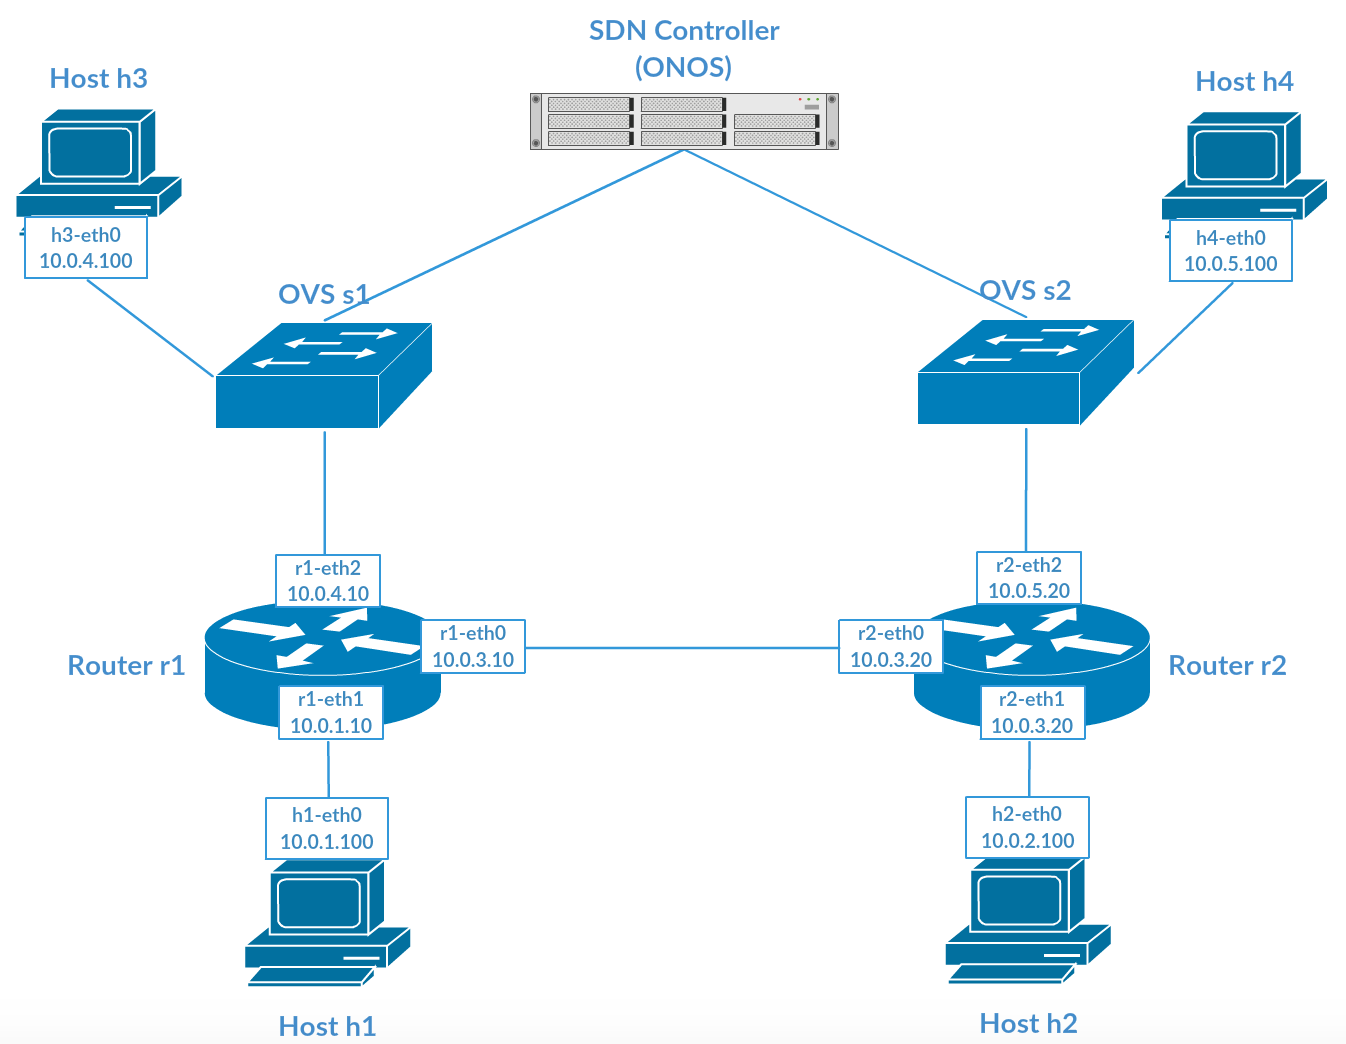
\includegraphics[width=0.8\textwidth]{./Figure/Topo/Exp3.png}
\caption{Ping Test on SDN and Non-SDN Combination Experiment \label{fig:Exp3}}
\end{figure}

\subsubsection{Edit OSPF Configuration
Files:}\label{edit-ospf-configuration-files}

\begin{quote}
\$ cd /usr/local/etc
\end{quote}

\begin{quote}
\$ sudo nano r1ospfd.conf
\end{quote}

\begin{adjustwidth}{1cm}{0cm}
\begin{verbatim}
hostname r1_ospfd
password 123
enable password 123

router ospf
  ospf router-id 10.0.3.10
  network 10.0.3.0/24 area 0
  network 10.0.1.0/24 area 0
  network 10.0.4.0/24 area 0
debug ospf event
log file /usr/local/etc/r1ospfd.log
\end{verbatim}
\end{adjustwidth}

\begin{quote}
\$ sudo nano r2ospfd.conf
\end{quote}

\begin{adjustwidth}{1cm}{0cm}
\begin{verbatim}
hostname r2_ospfd
password 123
enable password 123

router ospf
  ospf router-id 10.0.3.20
  network 10.0.3.0/24 area 0
  network 10.0.2.0/24 area 0
  network 10.0.5.0/24 area 0
debug ospf event
log file /usr/local/etc/r2ospfd.log
\end{verbatim}
\end{adjustwidth}

\subsubsection{Run Mininet Script:}\label{run-mininet-script}

\begin{quote}
\$ sudo python QuaggaOSPF (SDN+NONSDN).py
\end{quote}

\subsubsection{Ping Test:}\label{ping-test-2}

\begin{quote}
mininet\textgreater{} pingall
\end{quote}

It may take a while(40s) to add route.

\subsection{Trouble Shooting}\label{trouble-shooting}

\subsubsection{OSPF service wait a long time before adding
route.}\label{ospf-service-wait-a-long-time-before-adding-route.}
